\section{Introduction aux graphes}

\subsection{Vocabulaire des graphes}

\begin{defi}{Graphe}%\cite{ref_01}
Un graphe est un ensemble de \textbf{sommets} et  \textbf{relations} entre ces sommets.

Lorsque deux sommets sont en relation, on dit qu'il existe une \textbf{arête} entre ces sommets.
\end{defi}

\begin{defi}{Graphe non orienté -- Arêtes}
Un graphe non orienté $G$ est un couple $G=(S,A)$, où $S$ est un ensemble fini de sommets (appelés aussi n\oe uds)  et où $A$ est un ensemble fini de paires ordonnées de sommets, appelées arêtes.

On note $x - y$ l'arête $\{x,y\}$. $x$ et $y$ sont les deux extrémités de l'arête.
\end{defi}

\begin{defi}{Graphe orienté -- Arcs}\cite{ref_01}
Un graphe orienté $G$ est un couple $G=(S,A)$, où $S$ est un ensemble fini de sommets et où $A$ est un ensemble fini de paires ordonnées de sommets, appelées arcs.

On note $x\to y$ l'arc $(x,y)$. $x$ est l'extrémité initiale de l'arc, $y$ est son extrémité terminale. On dit que $y$ est successeur de $x$ et que $x$ est prédécesseur de $y$. 
\end{defi}

\begin{multicols}{2}
\begin{figure}[H]
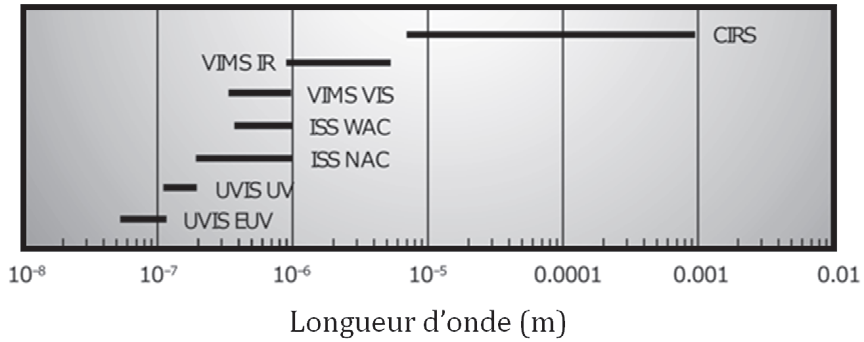
\includegraphics[width=.8\linewidth]{fig_02}
\captionsetup{justification=centering}
\caption{Graphe non orienté \label{fig_02}}
\end{figure}

\begin{figure}[H]
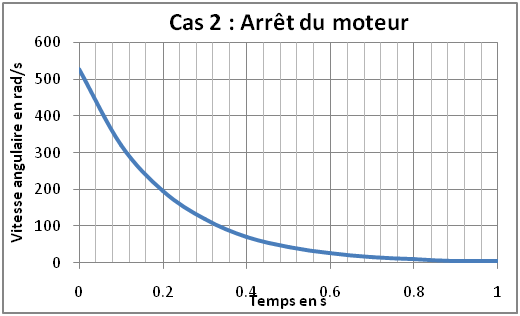
\includegraphics[width=.8\linewidth]{fig_03}
\captionsetup{justification=centering}
\caption{Graphe orienté}
\end{figure}
\end{multicols}

\begin{rem}
On peut noter le graphe non orienté $G=\left(\llbracket 1,6\rrbracket,E\right)$ où $E=\left(
\left\{1,2\right\},\left\{2,3\right\},\left\{3,4\right\},\left\{1,4\right\},\left\{1,3\right\},\left\{1,5\right\},\left\{1,6\right\}\right)$ désigne les arêtes. 

On peut noter le graphe orienté $G=\left(\llbracket 1,6\rrbracket,E\right)$ où $E=\left(
\left(1,2\right),\left(2,3\right),\left(3,4\right),\left(1,4\right),\left(1,3\right),\left(1,5\right),\left(1,6\right)\right)$ désigne les arcs. 
\end{rem}

\begin{defi}{Adjacence}
Deux arcs (resp. arêtes) d'un graphe orienté (resp. non orienté) sont dits adjacents s'ils ont au moins une extrémité commune. 

Deux sommets d'un graphe non orienté sont dits adjacents s'il existe une arête les joignant. 

Dans un graphe orienté, le sommet $y$ est dit adjacent au sommet $x$ s'il existe un arc $x\to y$.
\end{defi}


\begin{defi}{Graphes pondérés}
Étiqueter les arêtes d’un graphe $(S, A)$ (orienté ou non), c’est se donner une fonction
$f : A \to V$ (où $V$ est un ensemble de valeurs). On dit qu’un graphe est pondéré si ses arêtes sont étiquetées par des nombres. On parlera alors du poids d’une arête.
\end{defi}
%
%\begin{defi}{Sommet (ou n\oe{}uds)}
%\end{defi}
%
%\begin{defi}{Arc, arête}
%\end{defi}

\subsection{Chermins}

\begin{defi}{Chemin dans un graphe}
On appelle chemin dans un graphe une suite finie $\{S_0, \ldots , S_{n-1}\}$ de $n$ sommets tels que pour tout
$i \in \llbracket 0, n-1\llbracket$, une arête relie $S_i$ à $S_{i+1}$. On dit que ce chemin relie le sommet de départ $S_0$ au sommet de fin $S_{n-1}$. 

Dans le cas d'un graphe non orienté, les arêtes sont notées $\{S_i, S_{i+1}\}$ pour $i \in \llbracket 0, n-1\llbracket$.

Dans le cas d'un graphe orienté, les arêtes sont notées $(S_i, S_{i+1})$ pour $i \in \llbracket 0, n-1\llbracket$.
\end{defi}


\begin{defi}{Chemin fermé}
Chemin dont le sommet de départ et le sommet d'arrivé sont identiques.
\end{defi}

\begin{defi}{Chemin élémentaire}
Chemin n'empruntant que des arêtes distinctes.
\end{defi}

\begin{defi}{Chemin simple}
Chemin tel que les $n - 2$ sommets intermédiaires si, pour $i \in \llbracket 1, n-1\llbracket$ soient
deux à deux distincts et tous distincts du sommet de départ $S_0$ et du sommet d’arrivée $S_{n-1}$ et tels
que ce chemin n’est pas de la forme $a, b, a$ dans le cas non-orienté.
\end{defi}

\begin{defi}{Circuit}
Chemin fermé de longueur non nulle.
\end{defi}


\begin{defi}{Cycle}
Circuit élémentaire (chemin fermé de longueur non nulle dont toutes les arêtes sont distinctes).
\end{defi}

\begin{defi}{Cycle simple} 
Chemin fermé et simple de longueur non nulle.
\end{defi}

\begin{defi}{Chemin et cycle eulérien}
Chemin (resp. cycle) contenant une et une seule fois toutes les arêtes du graphe.
%Graphe eulérien : contenant un circuit eulérien.
%Graphe acyclique : ne contenant aucun cycle.
\end{defi}

\begin{rem}
Pour certains auteurs, un chemin élémentaire est ce que nous avons appelé un chemin simple et réciproquement. Pour d’autres, un cycle est ce que nous avons appelé un cycle simple.
\end{rem}

%\begin{defi}{}
%\end{defi}
%
%\begin{defi}{}
%\end{defi}



\begin{defi}{Connexité dans les graphes non orientés}
\end{defi}

\subsection{Notations}
\begin{defi}{Degré d'un sommet}
On appelle degré d'un sommet $s$ et on note $d\left(s\right)$ le nombres d'arcs (ou d'arêtes) dont $s$ est une extrémité.
\end{defi}

\begin{defi}{Degré entrant et sortant}
On note $s$ le sommet d'un graphe orienté. On note : 
\begin{itemize}
\item $d_{+}\left(s\right)$ le demi-degré extérieur de $s$, c'est-à-dire le nombre d'arcs ayant leur extrémité initiale en $s$ (ces arcs sont dits incidents à $s$ vers l'extérieur);
\item $d_{-}\left(s\right)$ le demi-degré intérieur de $s$, c'est-à-dire le nombre d'arcs ayant leur extrémité finale en $s$ (ces arcs sont dits incidents à $s$ vers l'intérieur).
\end{itemize}

Dans ce cas, on a  $d\degres\left(s\right)=d_{-}\left(s\right)+d_{+}\left(s\right)$.
\end{defi}


\begin{exemple}~\\

\begin{multicols}{2}
\begin{figure}[H]
\centering
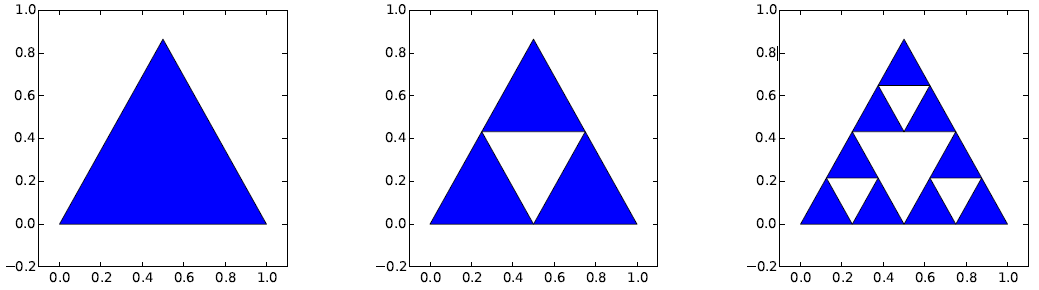
\includegraphics[width=.8\linewidth]{fig_04}
\captionsetup{justification=centering}
\caption{Graphe orienté \label{fig_04}}
\end{figure}

\begin{itemize}
\item $d_{-}\left(S_1\right)=3$.
\item $d_{+}\left(S_1\right)=4$.
\item $d\degres\left(S_1\right)=7$.
\end{itemize}
\end{multicols}

\end{exemple}

\subsection{Implémentation des graphes}

\subsubsection{Liste d'adjacence}
\begin{defi}{Liste d'adjacence}
Soit un graphe de $n$ sommets d'indices $i \in \llbracket 0, n-1\rrbracket$. Pour implémenter le graphe, on utilise une liste \texttt{G} de taille $n$ pour laquelle, \texttt{G[i]} est la liste des voisins de \texttt{i}.
\end{defi}
\begin{rem}
Cette implémentation est plutôt réservée au graphes << creux >>, c'est-à-dire ayant peu d'arêtes.
\end{rem}

\begin{exemple} ~\\
\begin{minipage}[b]{.47\linewidth}
\begin{center}
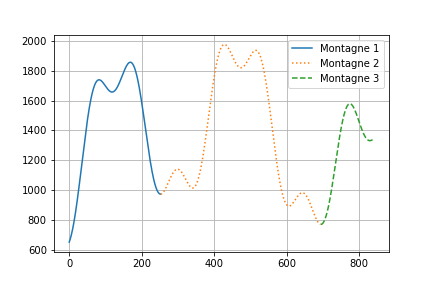
\includegraphics[width=.7\linewidth]{fig_05}
\end{center}
Dans ce cas $S_0$ est voisin de $S_1$, $S_5$ et $S_6$; donc \texttt{G[0]=[1,5,6]}. 
$S_3$ est voisin de $S_2$ et $S_4$; donc \texttt{G[3]=[2,4]}.
\begin{lstlisting}
G = [[1,5,6],[0,2,6],[1,3],[2,4],[3,5],
      [4,0],[1,0]]
\end{lstlisting}
\end{minipage}\hfill
\begin{minipage}[b]{.47\linewidth}
\begin{center}
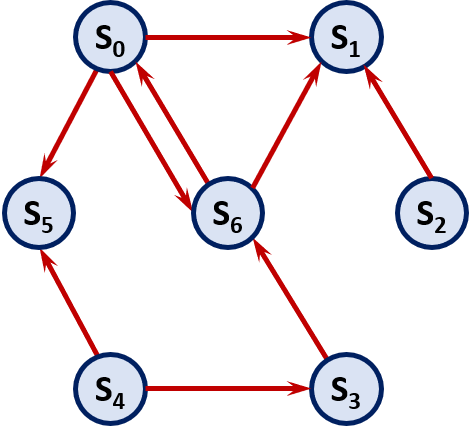
\includegraphics[width=.7\linewidth]{fig_06}
\end{center}
Dans ca cas, le graphe est orienté. La liste d'adjacence contient la liste des successeurs. Ainsi, les successeurs de $S_0$ sont $S_1$, $S_5$ et $S_6$; donc \texttt{G[0]=[1,5,6]}. $S_1$ n'a pas de successeur donc \texttt{G[1]=[]}.
\begin{lstlisting}
G = [[1,5,6],[],[1],[6],[3,5],[],[0,1]]
\end{lstlisting}
\end{minipage}


Dans la même idée, il est aussi possible d'utiliser des dictionnaires d'adjacence dans lequel les clés sont les sommets, et les valeurs sont des listes de voisins ou de sucesseurs. 
\begin{lstlisting}
# Graphe non orienté 
G = {"S0":["S1","S5","S6"],"S1":["S0","S2","S6"],"S2":["S1","S3"],"S3":["S2","S4"],"S4":["S3","S5"],"S5":["S4","S0"],"S6":["S1","S0"]}
# Graphe orienté 
G = {"S0":["S1","S5","S6"],"S1":[],"S2":["S1"],"S3":["S6"],"S4":["S3","S5"],"S5":[],"S6":["S1","S0"]}
\end{lstlisting}

\end{exemple}

\subsubsection{Matrice d'adjacence}
\begin{defi}{Matrice d'adjacence}
Soit un graphe de $n$ sommets d'indices $i \in \llbracket 0, n-1\rrbracket$ et $E$ l'ensemble des arêtes 
(on notera $G=\left( \llbracket 0, n-1\rrbracket,E\right)$. Pour implémenter le graphe, on utilise la matrice d'adjacence carrée de taille $n$, $\mathcal{M}_n$ \texttt{G} de taille $n$ pour laquelle,
$m_{i,j}=\left\{
\begin{array}{l}
\texttt{True } \text{ si } \{i,j\}\in E\\
\texttt{False } \text{ sinon } 
\end{array}
\right.$ avec $i,j\in \llbracket 0, n-1\rrbracket$. 


\end{defi}
\begin{rem}
Cette implémentation est plutôt réservée au graphes << denses >> ayant << beaucoup >> d'arêtes.
\end{rem}


\begin{exemple} ~\\
\begin{minipage}[b]{.47\linewidth}
\begin{center}
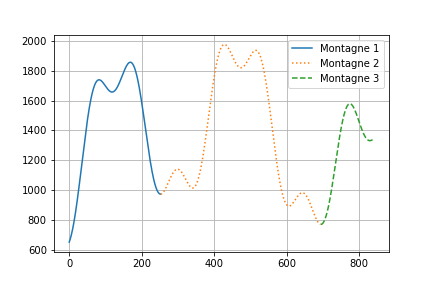
\includegraphics[width=.7\linewidth]{fig_05}
\end{center}

On a dans ce cas 

\footnotesize{$
M = $

$
\begin{pmatrix}
\texttt{False} & \texttt{True} & \texttt{False} & \texttt{False} & \texttt{False} & \texttt{True} & \texttt{True} \\
\texttt{True} & \texttt{False} & \texttt{True} & \texttt{False} & \texttt{False} & \texttt{False} & \texttt{True} \\ 
\texttt{False} & \texttt{True} & \texttt{False} & \texttt{True} & \texttt{False} & \texttt{False} & \texttt{False} \\
\texttt{False} & \texttt{False} & \texttt{True} & \texttt{False} & \texttt{True} & \texttt{False} & \texttt{False} \\
\texttt{False} & \texttt{False} & \texttt{False} & \texttt{True} & \texttt{False} & \texttt{True} & \texttt{False} \\
\texttt{True} & \texttt{False} & \texttt{False} & \texttt{False} & \texttt{True} & \texttt{False} & \texttt{False} \\
\texttt{True} & \texttt{True} & \texttt{False} & \texttt{False} & \texttt{False} & \texttt{False} & \texttt{False} \\
\end{pmatrix}$}

ou 

\footnotesize{$
M = 
\begin{pmatrix}
\texttt{0} & \texttt{1} & \texttt{0} & \texttt{0} & \texttt{0} & \texttt{1} & \texttt{1} \\
\texttt{1} & \texttt{0} & \texttt{1} & \texttt{0} & \texttt{0} & \texttt{0} & \texttt{1} \\ 
\texttt{0} & \texttt{1} & \texttt{0} & \texttt{1} & \texttt{0} & \texttt{0} & \texttt{0} \\
\texttt{0} & \texttt{0} & \texttt{1} & \texttt{0} & \texttt{1} & \texttt{0} & \texttt{0} \\
\texttt{0} & \texttt{0} & \texttt{0} & \texttt{1} & \texttt{0} & \texttt{1} & \texttt{0} \\
\texttt{1} & \texttt{0} & \texttt{0} & \texttt{0} & \texttt{1} & \texttt{0} & \texttt{0} \\
\texttt{1} & \texttt{1} & \texttt{0} & \texttt{0} & \texttt{0} & \texttt{0} & \texttt{0} \\
\end{pmatrix}$}


\end{minipage}\hfill
\begin{minipage}[b]{.47\linewidth}
\begin{center}
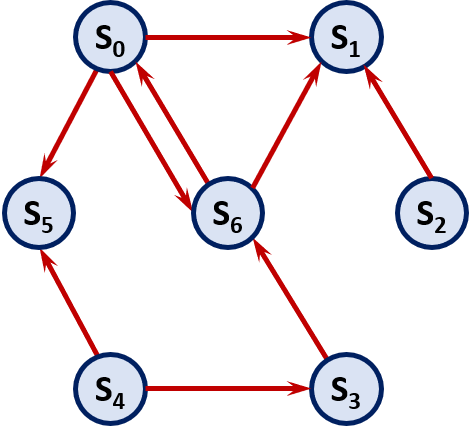
\includegraphics[width=.7\linewidth]{fig_06}
\end{center}
Dans ca cas, le graphe est orienté. On a 
On a dans ce cas 

\footnotesize{$
M = $

$
\begin{pmatrix}
\texttt{False} & \texttt{True} & \texttt{False} & \texttt{False} & \texttt{False} & \texttt{False} & \texttt{True} \\
\texttt{False} & \texttt{False} & \texttt{False} & \texttt{False} & \texttt{False} & \texttt{False} & \texttt{False} \\ 
\texttt{False} & \texttt{True} & \texttt{False} & \texttt{False} & \texttt{False} & \texttt{False} & \texttt{False} \\
\texttt{False} & \texttt{False} & \texttt{False} & \texttt{False} & \texttt{False} & \texttt{False} & \texttt{True} \\
\texttt{False} & \texttt{False} & \texttt{False} & \texttt{True} & \texttt{False} & \texttt{True} & \texttt{False} \\
\texttt{False} & \texttt{False} & \texttt{False} & \texttt{False} & \texttt{False} & \texttt{False} & \texttt{False} \\
\texttt{True} & \texttt{True} & \texttt{False} & \texttt{False} & \texttt{False} & \texttt{False} & \texttt{False} \\
\end{pmatrix}$}

ou 
\footnotesize{$
M =
\begin{pmatrix}
\texttt{0} & \texttt{1} & \texttt{0} & \texttt{0} & \texttt{0} & \texttt{0} & \texttt{1} \\
\texttt{0} & \texttt{0} & \texttt{0} & \texttt{0} & \texttt{0} & \texttt{0} & \texttt{0} \\ 
\texttt{0} & \texttt{1} & \texttt{0} & \texttt{0} & \texttt{0} & \texttt{0} & \texttt{0} \\
\texttt{0} & \texttt{0} & \texttt{0} & \texttt{0} & \texttt{0} & \texttt{0} & \texttt{1} \\
\texttt{0} & \texttt{0} & \texttt{0} & \texttt{1} & \texttt{0} & \texttt{1} & \texttt{0} \\
\texttt{0} & \texttt{0} & \texttt{0} & \texttt{0} & \texttt{0} & \texttt{0} & \texttt{0} \\
\texttt{1} & \texttt{1} & \texttt{0} & \texttt{0} & \texttt{0} & \texttt{0} & \texttt{0} \\
\end{pmatrix}$}

\end{minipage}
\end{exemple}


\begin{rem}
\begin{itemize}
\item Dans le cas d'un graphe non orienté, la matrice est symétrique. 
\item Si on avait un bouclage sur un sommet, il y aurait des valeurs non nulles sur la diagonale. 
\end{itemize}
\end{rem}

\section{Parcours d'un graphe}
\subsection{Piles et files}


\subsusection{Pile}
\begin{defi}{Pile}
Une pile est une structure de données dans laquelle le dernier élément stocké est le premier à en sortir. On parle de principe \textit{LIFO} pour \textit{Last In First Out}. Le dernier élément stocké est appelé \textbf{sommet}.
\end{defi}

Pour gérer une pile, indépendamment de la façon dont elle est implémentée, on suppose exister les opérations élémentaire suivantes : 
\begin{itemize}
\item création d'une pile vide;
\item test si une est vide;
\item rajout d'un élément au sommet de la pile;
\item accès au sommet d'une pile non vide;
\item suppression (et renvoi) du sommet d'une pile non vide.
\end{itemize}

Théoriquement, chacune de ces opérations doit se faire à \textbf{temps constant}. 

\subsection{Parcours générique d'un graphe}

\subsection{Parcours en largeur}

\subsection{Parcours en profondeur}

\subsection{Détection de la présence des cycles}

\subsection{Connexité d'un graphe non orienté}

\section{Pondération d'un graphe}



\section{Recheche du plus court chemin}
\subsection{Algorithme de Dijkstra}

\subsection{Algorithme A$\star$}

\begin{defi}{}
\end{defi}

\begin{defi}{}
\end{defi}

\begin{defi}{}
\end{defi}

\begin{defi}{}
\end{defi}

\begin{defi}{}
\end{defi}
